\documentclass[UTF8]{ctexart}
% \usepackage{amsfonts}
% \usepackage{amsmath}
% \usepackage{amssymb}
% \usepackage{amsthm}
% \usepackage{booktabs}
\usepackage{courier}
% \usepackage{float}
\usepackage{geometry}
\usepackage{graphicx}
\usepackage{hyperref}
% \usepackage{listings}
\geometry{left=2.54cm,right=2.54cm,top=2.18cm,bottom=3.18cm}

\begin{document}

\title{人脸表情识别报告}
\author{无46\ \ 黄秀峰\ \ 2014011193\\ 无46\ \ 严靖凯\ \ 2014011192\\ 无46\ \ 王启睿\ \ 2014011179}
\maketitle

\section{概述}

对于人脸表情识别问题,目前学术界已有了一定的研究,并且当前在该问题上有许多算法比赛,吸引着众多科研人员参与。比较典型的包括Kaggle的FERC,SSPNET的FERA,ACM的EmotiW,等等。这些比赛采用特定的数据集,有一些由实验室环境下采集的数据为主,另一些直接来自于实际图片或视频。

在本报告中,我们将首先说明我们选用的方法及原因,再对算法实现进行介绍,最后对判别结果进行分析,并指出可能的未来改进方向。

\section{选用方法的确定}

本节中,我们将介绍我们曾着重考虑过的两种方法以及最终选用方法的确定。其中一是采用WLD+HOG特征的传统模式识别方法,二是采用神经网络的特征提取识别方法。

\subsection{两种思路}

与目前大多数机器学习问题一样,对与人脸表情识别问题的处理方法,大体可分为传统模式识别和神经网络两类。其中,传统模式识别方式的代表性文章有
\cite{happy2015automatic,islam2016sention,wang2013feature,salmam2016facial}等,其中大多数采用SVM或决策树进行判决,神经网络方式的代表性文章有
\cite{BarsoumICMI2016,khorrami2015deep}等。传统方法往往训练和运行速度很快,部分方法甚至可以应用于实时视频流作为输入等场景,对于质量高(清晰、光照合适、正脸)的图片有很高的识别正确率;而神经网络方法对于很低的图片分辨率、不理想的光照、侧脸,或视频片段等情形的处理效果较好。

在我们本次实验任务中,我们面对两个主要挑战:一是需要对自采数据集进行判决,其中的图片与实验室中标准数据有很大区别;二是本次提供的训练图片数很少,只有521张。前者促使我们考虑神经网络的方法,但后者使得神经网络的训练条件不足。相比之下,传统方法在小数据样本情形下通常有更好的效果。

\subsection{神经网络的尝试}
根据我们所调研的文献,文章\cite{BarsoumICMI2016}提供的FER+数据集中有较多数据,因此我们选择在FER+数据集上复现文\cite{BarsoumICMI2016}的效果。

\begin{figure}[ht]
  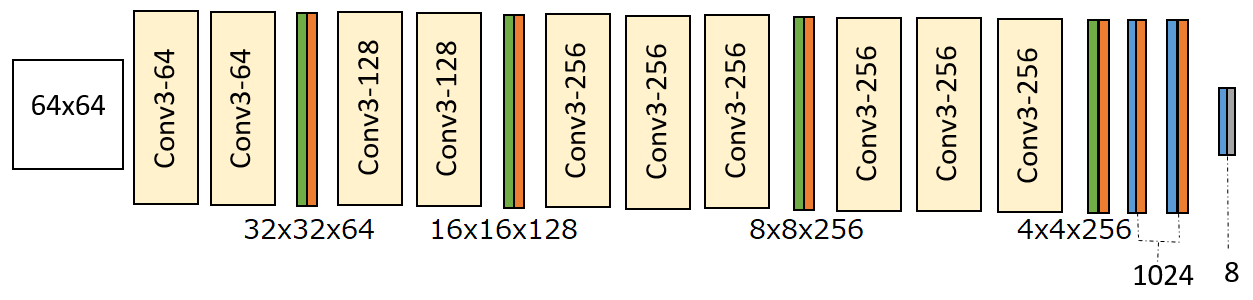
\includegraphics[width=\textwidth]{ferplus.png}
  \caption{测试使用的CNN结构}\label{fig:ferplus}
\end{figure}

整个网络结构如上图所示,输入为为$64\times 64$灰度图片,其后的黄、绿、橙、蓝、灰色分别对应于卷积层、最大池化层、Dropout层、全连接+ ReLU层、Softmax层。该网络自VGG-13修改而来,以适应低分辨率的FER数据集。
训练得到的准确率在85\% 左右,与文中得到的结果基本一致。
事实上,该准确率很大程度上是受FER+数据集自身所限。FER+数据集使用$64\times 64$的8bit灰度图片,且包含各种姿势(如侧脸、捂脸等),相比本次实验中最终需要测试的CK+、JAFFE等高分辨率正脸数据集而言,识别难度难度更大。针对前述测试数据集,下文提到的传统方法能够在更短时间、更小训练集下取得相仿甚至更高的正确率。

然而,仅仅在\cite{BarsoumICMI2016}中采用的数据集上达到这一准确率是远远不够的。我们用实验提供的训练数据进行了测试,发现判决效果并不理想,准确率较低。因此我们转而考虑采用传统的特征提取方式,在下文中将详细介绍。

\section{算法实现}

\subsection{预处理}

% 有没有啊  没有就不要

\subsection{WLD特征提取}

\subsection{HOG特征提取}

\subsection{最近邻判定}

\section{实验结果}

\subsection{准确率}

%%%%%%%%%%%%%%%%%%%%%%%%%%%%%%%%%%%%%
%
% 对于为什么我们得到的准确率在自采和标准上差不多,有什么好的解释吗……我想不出来T^T
%
%%%%%%%%%%%%%%%%%%%%%%%%%%%%%%%%%%%%%

\subsection{错判样例与分析}

\section{总结}

对于本实验,我们采用WLD+HOG特征提取及最近邻判别的方法完成了判决的过程。得到的准确率属于中等,还有较大的改进空间。我们目前看来,主要的改进方式包括以下几点:
\begin{itemize}
  \item 增加模型训练集的大小,用更全面、更具有代表性的样本进行训练。
  \item 尝试采用其他图像特征。我们曾尝试过采用LBP特征,但效果并不好,因此最后将该部分舍弃。如果未来有更加合适的图像特征提取方式被提出,可以考虑采用。
  \item 当训练样本足够大时,可以考虑重新采用神经网络训练的方法,应该可以显著提高准确率。
\end{itemize}

总之,经过本次实验,我们对人脸表情识别这一当前热门问题有了更加深入的了解,同时也动手实现了图像特征提取、分类、神经网络等多种机器学习的常用方法,能力得到了极大的锻炼。

最后,衷心感谢老师和助教一学期以来的付出!

\bibliographystyle{unsrt}
\bibliography{finalref}

\end{document}
